%----------------------------------------------------------------------------------------
%	PACKAGES AND THEMES
%----------------------------------------------------------------------------------------
\documentclass[aspectratio=169,xcolor=dvipsnames]{beamer}
\usetheme{Simple}

\usepackage{hyperref}
\usepackage{graphicx} % Allows including images
\usepackage{booktabs} % Allows the use of \toprule, \midrule and \bottomrule in tables

%----------------------------------------------------------------------------------------
%	TITLE PAGE
%----------------------------------------------------------------------------------------

% The title
\title[short title]{Can We Use FIFA Videogame Data in Soccer Analytics?}
\subtitle{Statistical Learning Project}

\author {Alvise Dei Rossi\footnote{ID: 2004250} - Lorenzo Corrado\footnote{ID: 2020623} - Riccardo Vinco\footnote{ID: 2005800}}

\institute[UNIPD] % Your institution may be shorthand to save space
{
    % Your institution for the title page
    Department of Mathematics "Tullio Levi-Civita" \\
    MS in Data Science \\
    University of Padua
    \vskip 3pt
}
\date{A.Y. 2020/2021} % Date, can be changed to a custom date

%----------------------------------------------------------------------------------------
%	PRESENTATION SLIDES
%----------------------------------------------------------------------------------------

\begin{document}

%------------------------------------------------

\begin{frame}
    % Print the title page as the first slide
    \titlepage
\end{frame}

\begin{frame}{Overview}
    % Throughout your presentation, if you choose to use \section{} and \subsection{} commands, these will automatically be printed on this slide as an overview of your presentation
    \tableofcontents
\end{frame}

%------------------------------------------------

\section{Introduction}

%------------------------------------------------
\begin{frame}{Introduction}
\begin{itemize}
    \item Soccer is the most popular sport in the world, both for the number of players and for the number of spectators. The soocer industry is worth about \$471 billion in 2018 and predictions say it will be worth about \$600 billion in 2025 \cite{1}
    
    \item Despite the huge following that this sport has and the large number of spectators, analysts and professionals, it is still very difficult to make predictions in football, both for the absence of adequate datasets and for the intrinsic difficulty in modeling events in this sport \cite{2}
    
    \item Given the enormous success that this sport has over time, several simulation video games have been developed.
\end{itemize}
\end{frame}

%------------------------------------------------

\begin{frame}{Introduction - II}
\begin{itemize}
\item FIFA 20 is the most popular football video game, developed by EA Sports, available for the major videogame consoles. The video game is distributed all over the world and sold, in the year 2020, about 115 million copies for a billionaire turnover.
\end{itemize}
\begin{figure}[H] 
\begin{center} 
  % Requires \usepackage{graphicx} 
  
\includegraphics[width=7.5cm]{fifa20.jpg}\\ 
  % \caption{} 
\end{center} 
\end{figure}
\end{frame}

%------------------------------------------------

\begin{frame}{Introduction - III}
\begin{itemize}
\item To ensure a high quality simulation, EA Sports uses a large number of soccer scouts for the evaluation of the characteristics and attributes for players from all over the world, but this characterization of the players is a difficult job

\item The aim of this project is to establish if there is a relationship (and how strong it is) between the player's in-game statistics with the real world

% \item As we can see each attribute goes from 0 to 100

\item We believe that in-game statistics can also be a very important data resource for many statistical analysis applications in soccer
\end{itemize}
\end{frame}

%------------------------------------------------

\begin{frame}{Introduction - IV}
\begin{itemize}

\item A professional soccer player is assigned a series of statistics, more than 20, that are representative of his in-real characteristics and consider all the major leagues in the world.
\end{itemize}
\begin{figure}[H] 
\begin{center} 
  % Requires \usepackage{graphicx} 
  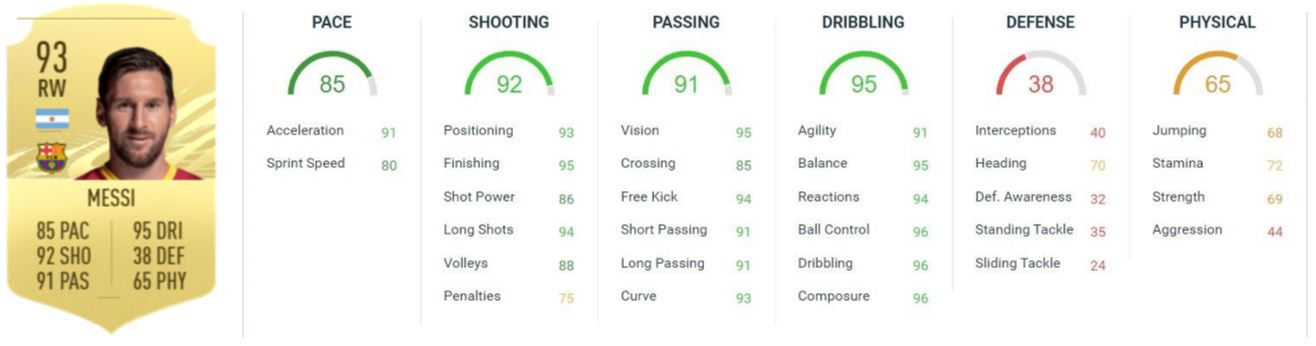
\includegraphics[width=13.5cm]{fine.jpg}\\ 
  % \caption{} 
\end{center} 
\end{figure}
\begin{itemize}

\item The quality of the estimation of these characteristics is fundamental in a soccer simulation game. Player stats are therefore expected to be consistent with the real world. 
\end{itemize}
\end{frame}

%------------------------------------------------

\section{Data and Preprocessing}

%------------------------------------------------
\begin{frame}{Data and Preprocessing}
\begin{itemize}

    \item The FIFA 21 dataset we used contains 18,944 players, on which 106 variables were measured. For example, players are represented by:
\end{itemize}
\begin{small}
\begin{table} [ht]
\centering
\begin{tabular}{ccccccccc} 
  \hline
    & sofifa\_id & short\_name & age & height\_cm & weight\_kg & nationality & \dots \\
    \hline
    1 & 158023 & L. Messi &  33 & 170 &  72 & Argentina & \dots\\ 
    \dots & &  &  & \dots &  & & \dots \\ 
    16 & 202126 & H. Kane & 26 & 188 &  89 & England & \dots\\ 
    \dots & &  &  & \dots &  & & \dots \\ 
    18944 & 257936 & Song Yue & 28 & 185 & 79 & China PR & \dots\\
    \hline
\end{tabular}
\end{table}
\end{small}
\end{frame}

%------------------------------------------------

\begin{frame}{Data and Preprocessing}
\begin{small}
\begin{block}{Quantitative variables in the dataset}
\begin{table}[ht]
\centering
\begin{tabular}{cccccc}
    FIFA ID & Age & Height & Weight & League rank & Overall\\ 
    Potential & Value & Wage & Reputation & Weak foot & Skill moves\\
    Physic & Crossing & Finishing & Heading & Short passing & Volleys\\
    Dribbling & Curve & Fk accuracy & Long passing & Ball Control & Acceleration\\
    Sprint speed & Agility & Reactions & Balance& Shot power&  Jumping\\   
    Stamina & Strength & Long shots & Aggression & Interceptions& Positioning\\
    Vision&  Penalties & Composure & Standing tackle& Sliding tackle & Gk Diving\\
    Gk handling & Gk kicking& Gk positioning & Gk reflexes
\end{tabular}
\end{table}
\end{block}
\end{small}
\begin{small}
\begin{block}{Categorical variables in the dataset}
\begin{table}[ht]
\centering
\begin{tabular}{cccc}
  Short Name & Nationality & Club name & League name\\
  Player positions & Preferred foot & Work rate & Team position
\end{tabular}
\end{table}
\end{block}
\end{small}
\end{frame}

%------------------------------------------------

\section{Exploratory Data Analysis}

%------------------------------------------------

\begin{frame}{Frame Title}
\begin{figure}[H] 
\begin{center} 
  % Requires \usepackage{graphicx} 
  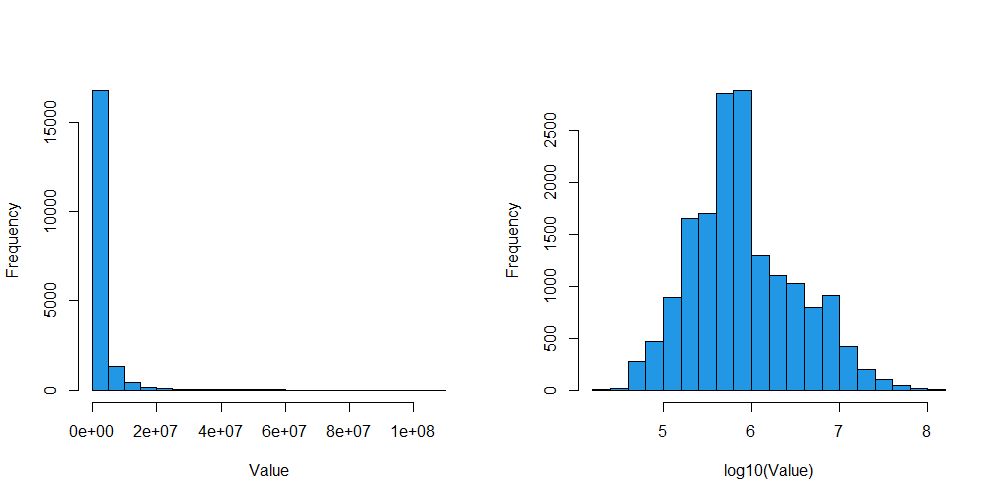
\includegraphics[width=12.5cm]{Rplot1.png}\\ 
  \caption{Valore} 
\end{center} 
\end{figure}
\end{frame}

%------------------------------------------------

\begin{frame}{Frame Title}
\begin{figure}[H] 
\begin{center} 
  % Requires \usepackage{graphicx} 
  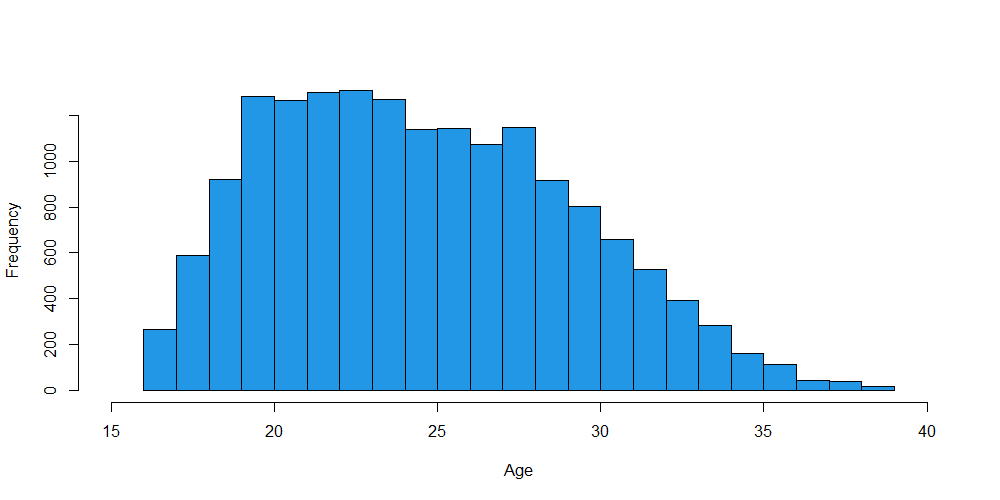
\includegraphics[width=11cm]{Rplot2.png}\\ 
  \caption{Età} 
\end{center} 
\end{figure}
\end{frame}

%------------------------------------------------

\begin{frame}{Frame Title}
\begin{figure}[H] 
\begin{center} 
  % Requires \usepackage{graphicx} 
  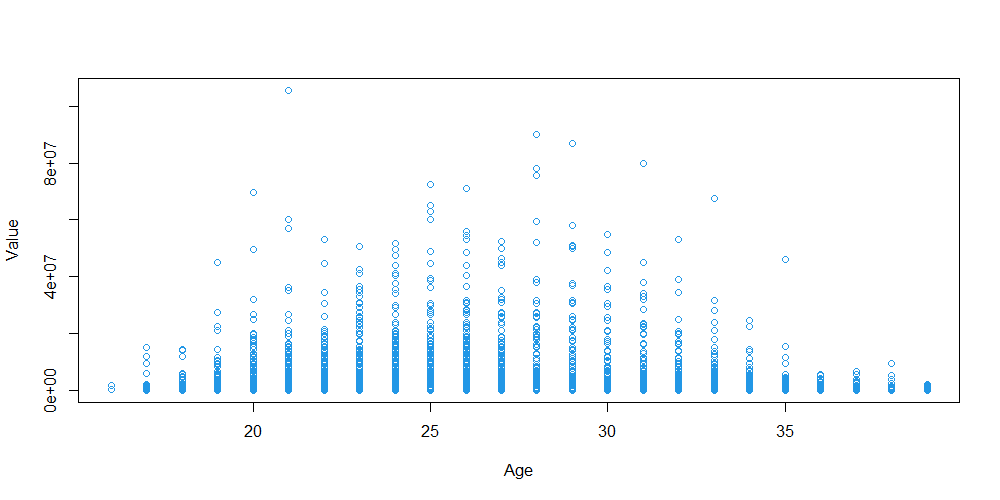
\includegraphics[width=11cm]{Rplot5.png}\\ 
  \caption{Età vs Valore} 
\end{center} 
\end{figure}
\end{frame}

%------------------------------------------------

\begin{frame}{Frame Title}
\begin{figure}[H] 
\begin{center} 
  % Requires \usepackage{graphicx} 
  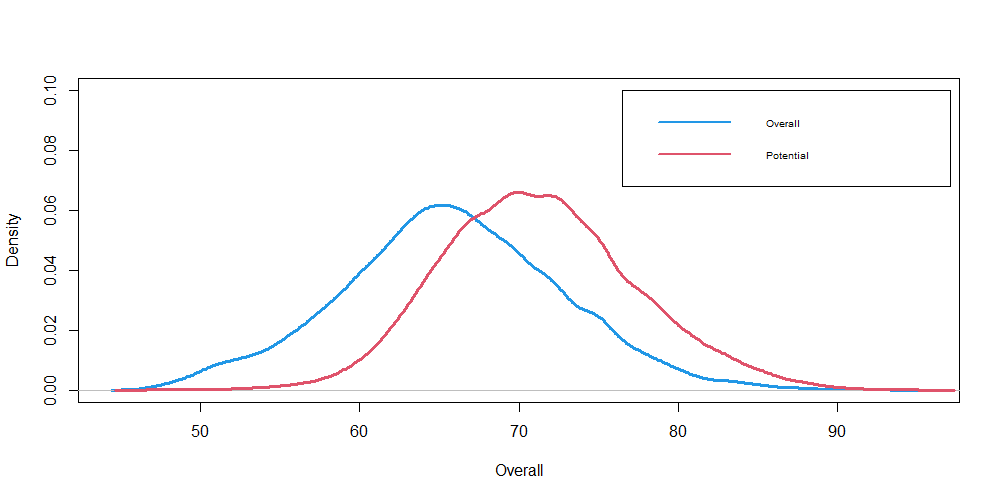
\includegraphics[width=11cm]{Rplot3.png}\\ 
  \caption{Overall} 
\end{center} 
\end{figure}
\end{frame}

%------------------------------------------------

\begin{frame}{Frame Title}
\begin{figure}[H] 
\begin{center} 
  % Requires \usepackage{graphicx} 
  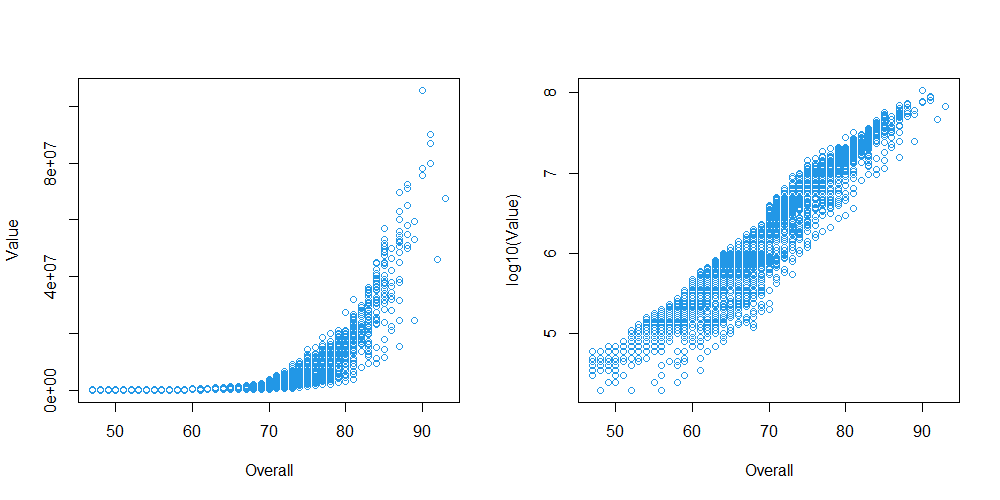
\includegraphics[width=11cm]{Rplot4.png}\\ 
  \caption{Overall vs Età} 
\end{center} 
\end{figure}
\end{frame}

%------------------------------------------------

\begin{frame}{Frame Title}
\begin{table}[ht]
\centering
\begin{tabular}{lccc}
  \hline
 Name & Value & Age & Overall \\ 
  \hline
  K. Mbappé & 105500000 &  21 &  90 \\ 
  Neymar Jr & 90000000 &  28 &  91 \\ 
  K. De Bruyne & 87000000 &  29 &  91 \\ 
  R. Lewandowski & 80000000 &  31 &  91 \\ 
  S. Mané & 78000000 &  28 &  90 \\ 
  M. Salah & 78000000 &  28 &  90 \\ 
  V. van Dijk & 75500000 &  28 &  90 \\ 
  R. Sterling & 72500000 &  25 &  88 \\ 
  H. Kane & 71000000 &  26 &  88 \\ 
  P. Dybala & 71000000 &  26 &  88 \\ 
   \hline
\end{tabular}
\caption{MVP}
\end{table}
\end{frame}

%------------------------------------------------

\begin{frame}{Frame Title}
\begin{figure}[H] 
\begin{center} 
  % Requires \usepackage{graphicx} 
  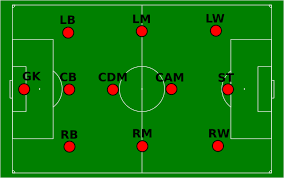
\includegraphics[width=9cm]{images.png}\\ 
  \caption{Positions} 
\end{center} 
\end{figure}
\end{frame}

%------------------------------------------------

\begin{frame}{Frame Title}
\begin{figure}[H] 
\begin{center} 
  % Requires \usepackage{graphicx} 
  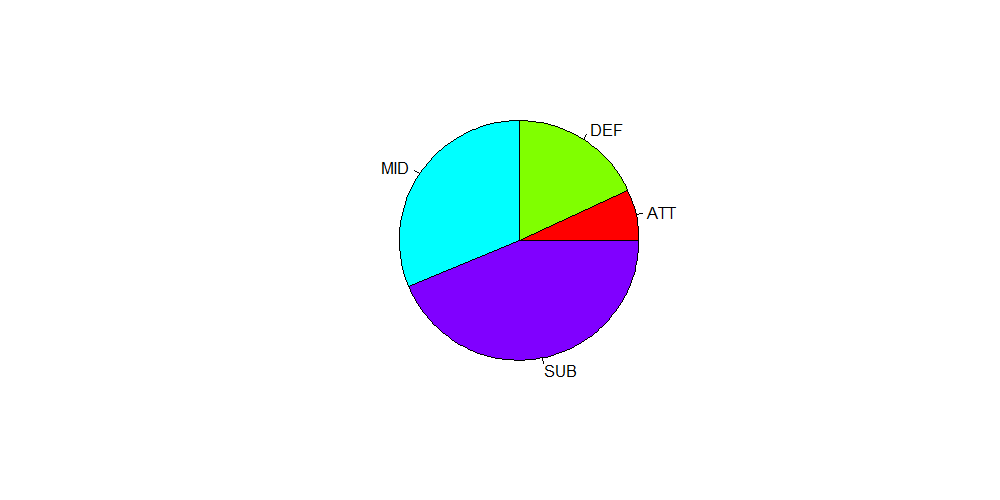
\includegraphics[width=15cm]{Rplot6.png}\\
\end{center} 
\end{figure}
\end{frame}

%------------------------------------------------
%allineamento tabella

\begin{frame}{Frame Title}
\begin{table}[ht]
\centering
\begin{tabular}{c|cccc}
    \hline
        DEF & GK & LB & CB & RB \\
        MID & CDM & CAM & LM & RM \\
        ATT & CF & LW & ST & RW  \\
    \hline
\end{tabular}
\caption{Positions in pie}
\end{table}
\end{frame}

%------------------------------------------------

\begin{frame}{Frame Title}
    
\end{frame}

%------------------------------------------------

\begin{frame}{Frame Title}
    
\end{frame}

%------------------------------------------------

\section{Models Estimation}

%------------------------------------------------

%------------------------------------------------

\begin{frame}{Models Estimation}
\begin{table}[ht]
\centering
\begin{tabular}{cc}
  \hline
    Categorical variables & Quantitative variables \\ 
  \hline
    International reputation & Overall \\ 
        & Potential \\ 
        & Age \\ 
   \hline
\end{tabular}
\caption{Predictors of Model 1 and Model 2}
\end{table}
\end{frame}

%------------------------------------------------

\begin{frame}{Models Estimation}
\begin{table}[ht]
\centering
\begin{tabular}{cc}
  \hline
    Categorical variables & Quantitative variables \\ 
  \hline
    International reputation & Overall \\ 
        & Potential \\ 
        & Age \\ 
   \hline
\end{tabular}
\caption{Predictors of Model 2.}
\end{table}
\end{frame}

%------------------------------------------------

\section{Interpretation}

%------------------------------------------------

\section{Applications}

%------------------------------------------------
\begin{frame}{}
    \centering
    \begin{Huge}
     Application 2: Soccer Predictions
    \end{Huge}
\end{frame}

\begin{frame}{The Elo rating system}
\begin{itemize}

    \item  The Elo is a score that is assigned to each team and which measures its strength, based on the results of previous matches
    
    \item This rating a system comes from the world of chess
    
    
    \begin{figure}[ht] 
        \begin{center} 
        % Requires \usepackage{graphicx} 
            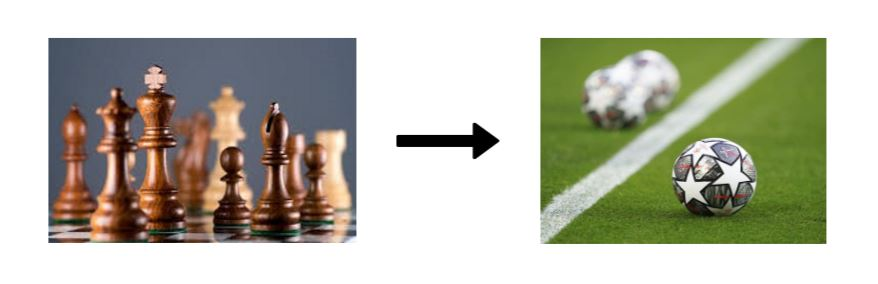
\includegraphics[width=12cm]{fre.jpg}\\
        \end{center} 
    \end{figure}
    
    \item The basic idea is to provide a summary measure of each team's strength, updating its score based on the result of each match.
    
    \item The variation depends on the strength of the team faced, if the victory takes place at home or not and the goal difference inflicted on the team faced.
\end{itemize}
\end{frame}

\begin{frame}{Elo update rule}
\begin{itemize}
 
    \item Considering $ l_0 ^ {H}, l_0 ^ {A} $ respectively the pre-match scores of the home team and the away team. On average, for the match in question it is assumed that the home and away teams mark:
    
    \begin{equation*}
        \gamma^{H} = \frac{1}{1+10^\frac{{l_0^{A} - l_0^{H}}}{400}}
        \hspace{2cm}
        \gamma^{A} = 1-\gamma^{H}
    \end{equation*}
    
    \item Considering the possible results, with reference to the home team:
    \begin{equation*}
        \alpha^H = 
        \begin{cases}
            1,$    if the home team won$ \\
            0.5,$    if the match war drawn$\\
            0, $    otherwise$
        \end{cases}
        \hspace{1cm}
        \alpha^A = 1-\alpha^H
    \end{equation*} 
    
    \item Team Elo ratings are updated after the end of each match via:
    \begin{equation*}
        l_1^H = l_0^H + 20(\alpha^H - \gamma^H) 
        \hspace{2cm}
        l_1^A = l_0^A + 20(\alpha^A - \gamma^A) 
    \end{equation*}
\end{itemize}
\end{frame}

%------------------------------------------------

\begin{frame}{Frame Title}
    \begin{itemize}
        \item This team rating system has been extensively studied and used to predict the outcome of many matches\cite{}
        \item The idea is to try to use the average Overall of the teams involved, instead of the Elo, in the match to estimate the probability of winning, drawing or losing
        \item However, to take into account the state of form of the teams we have decided to make the overall dynamic based on the trend of the Elo, for each team
    \end{itemize}
\end{frame}

%------------------------------------------------

\begin{frame}{Frame Title}
    \begin{figure}[ht] 
        \begin{center} 
        % Requires \usepackage{graphicx} 
            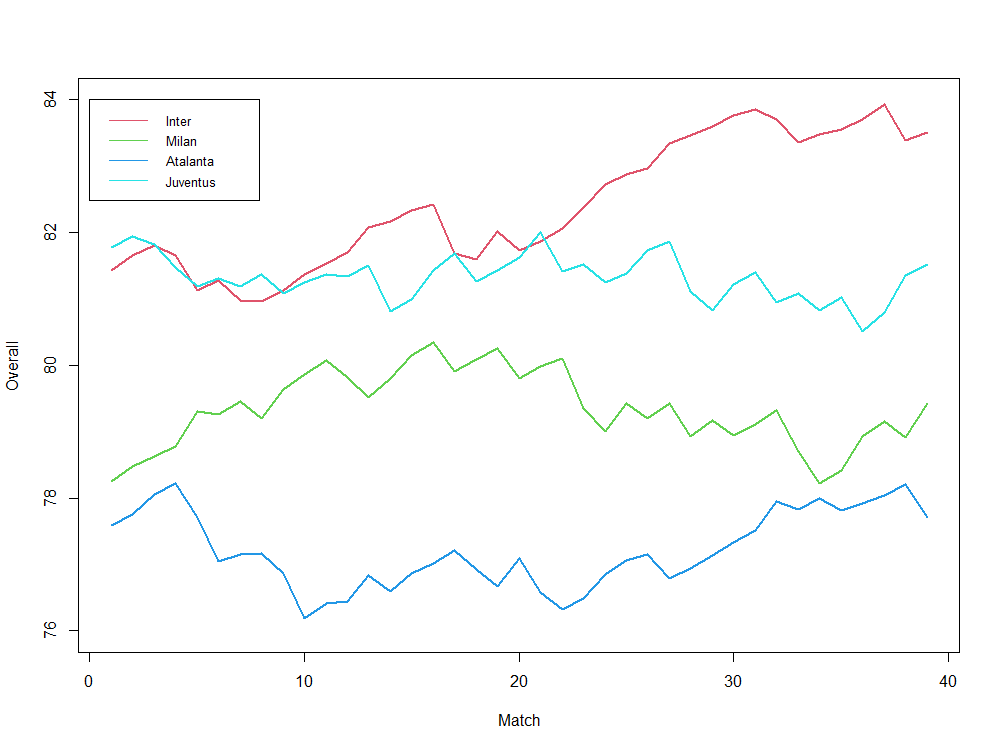
\includegraphics[width=7cm]{Rplot7.png}\\
         \caption{Elo}
        \end{center}
    \end{figure}
\end{frame}

%------------------------------------------------

\begin{frame}{Frame Title}
    \begin{itemize}
        \item To estimate a probability on the match result we use logistic regression in which we use as the only covariate variable:
        \begin{equation*}
            x = Overall^{H} - Overall^A
        \end{equation*}
        Then, the model is:
        \begin{equation*}
            log(\frac{p}{1-p}) = \alpha + \beta x + \epsilon
        \end{equation*}
        \item To have a comparison with this simple model, use the probability estimates provided during the championship by the bookmakers, in this case Betfair365 (B365)
    \end{itemize}
\end{frame}

%------------------------------------------------

\begin{frame}{Frame Title}
    \begin{figure}[ht] 
        \begin{center} 
        % Requires \usepackage{graphicx} 
            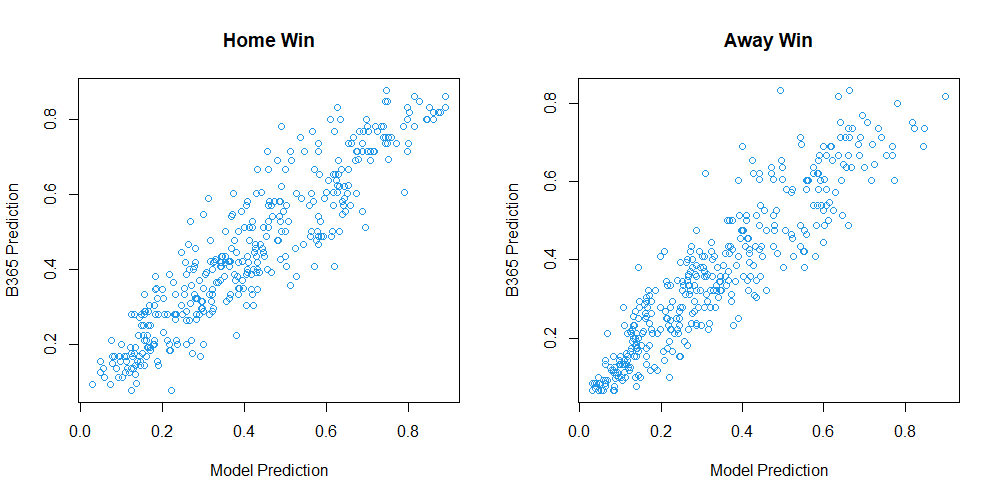
\includegraphics[width=11cm]{Rplot8.png}\\
         \caption{Prediction}
        \end{center}
    \end{figure}
\end{frame}

%------------------------------------------------

\begin{frame}{Possible improvements}
\begin{itemize}

    \item We only used the data relating to the 2020/2021 season only, we could obtain significant improvements by including data relating to more seasons
    
    \item We only used data from a single league, but by including data from multiple leagues the model estimates could improve considerably
    
    \item We only used the Overall as a parameter to estimate the team strength, we could use a different criterion for assigning the team's strength or a different criterion for the update
    
    \item Use different sources of data, also including statistics from real matches of the championship
\end{itemize}
\end{frame}

%------------------------------------------------

\section{Conclusions}

%------------------------------------------------

\section{References}

%------------------------------------------------

\begin{frame}[fragile] % Need to use the fragile option when verbatim is used in the slide
    \frametitle{Citation}
    An example of the \verb|\cite| command to cite within the presentation:\\~

    This statement requires citation \cite{p1}.
\end{frame}

%------------------------------------------------

\begin{frame}{References}
    % Beamer does not support BibTeX so references must be inserted manually as below
    \footnotesize{
        \begin{thebibliography}{99}
            \bibitem[Smith, 2012]{p1} John Smith (2012)
            \newblock Title of the publication
            \newblock \emph{Journal Name} 12(3), 45 -- 678.
        \end{thebibliography}
    }
\end{frame}

%------------------------------------------------

\begin{frame}
    \Huge{\centerline{The End}}
\end{frame}

%------------------------------------------------

\end{document}